\documentclass[border=10pt,crop=true]{standalone}
\usepackage{tikz}

\begin{document}
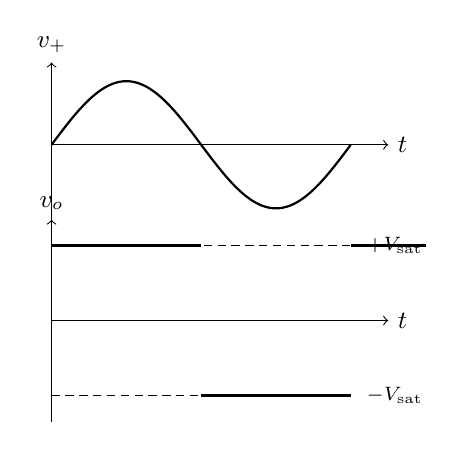
\begin{tikzpicture}[scale=0.95, font=\small]
  \def\T{4}
  \def\sat{1.0}

  \begin{scope}[shift={(0, 2.0)}]
    \draw[->] (0, 0) -- (\T+0.5, 0) node[right] {$t$};
    \draw[->] (0, -1.1) -- (0, 1.1) node[above] {$v_+$};
    \draw[thick, domain=0:\T, samples=120]
      plot (\x, {0.85*sin(360*\x/\T)});
  \end{scope}

  \begin{scope}[shift={(0, -0.35)}]
    \draw[->] (0, 0) -- (\T+0.5, 0) node[right] {$t$};
    \draw[->] (0, -1.35) -- (0, 1.35) node[above] {$v_o$};
    \draw[densely dashed] (0, \sat) -- (\T, \sat);
    \draw[densely dashed] (0, -\sat) -- (\T, -\sat);
    \node[font=\scriptsize, anchor=west] at (\T+0.08, \sat) {$+V_{\mathrm{sat}}$};
    \node[font=\scriptsize, anchor=west] at (\T+0.08, -\sat) {$-V_{\mathrm{sat}}$};
    \foreach \x/\y in {0/\sat, 1/\sat, 2/-\sat, 3/-\sat, 4/\sat} {
      \draw[very thick] (\x, \y) -- (\x+1, \y);
    }
  \end{scope}
\end{tikzpicture}
\end{document}
